% \chapter{Giới thiệu}
% \label{chap:chap1-introduce}

% Tại chương này, tác giả giới thiệu cấu trúc thư mục của dự án, giải thích các cài đặt, một số lưu ý trong quá trình sử dụng. Chương này cũng như báo cáo này không giới thiệu các cú pháp cơ bản như gõ phương trình, tạo bảng đơn giản, chèn hình ảnh.

% \section{Cấu trúc thư mục}

% \indent Hình \ref{fig:chap1-project-directory} mô tả cấu trúc thư mục của dự án. Thư mục \textbf{chapters} lưu các thành phần văn bản chính của dự án. Trong thư mục này chia làm ba thư mục, \textbf{\textit{back}} tương ứng với các phụ lục phía sau báo cáo.

% \begin{figure}
%     \centering
%     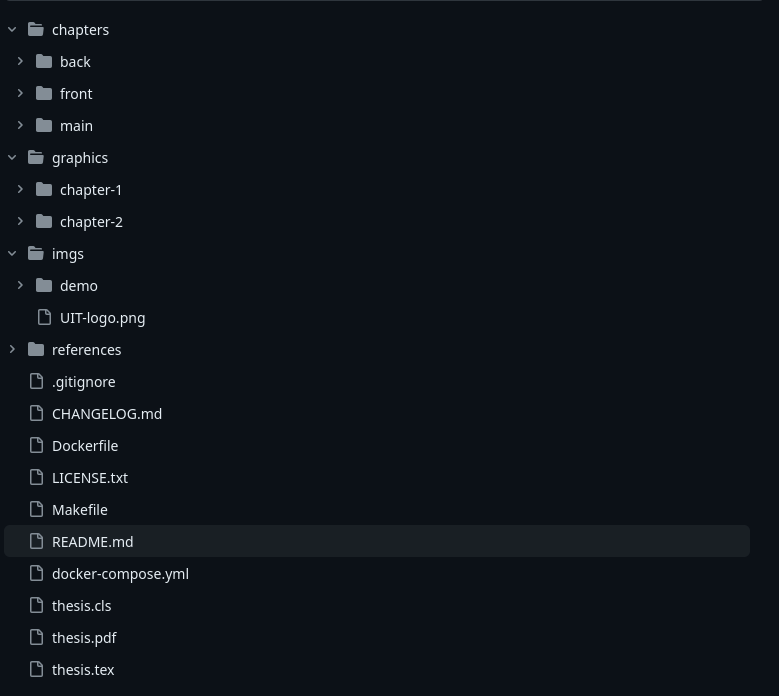
\includegraphics[scale=0.5]{chapter1/chap1-project-directory.png}
%     \caption{Cấu trúc thư mục của dự án}
%     \label{fig:chap1-project-directory}
% \end{figure}


% Thư mục \textbf{\textit{front}} tương ứng với các trang thông tin hội đồng chấm tốt nghiệp, lời cảm ơn, danh mục từ viết tắt... Thư mục \textbf{\textit{main}} chứa các chương của báo cáo. Báo cáo đánh số thứ tự riêng cho phần \textit{\textbf{front}}, trong khi phần các chương chính và phần phụ lục được đánh số giống nhau. Báo cáo đánh số trang bắt đầu từ trang tóm tắt, chữ số Ả-rập, bắt đầu bằng 1.

% Thư mục \textbf{\textit{graphics}} chứa hình ảnh được chèn vào báo cáo. Tương ứng với mỗi chương sẽ có 1 thư mục hình ảnh của chương đó.

% Thư mục \textbf{\textit{imgs}} là thư mục chứa hình ảnh của dự án, nó bao gồm các logo, watermark hoặc hình ảnh phục vụ cho document trên github. Hình chèn vào báo cáo không được lưu trong thư mục này.

% Thư mục \textbf{\textit{references}} chứa các file chỉ mục tài liệu tham khảo. Tương tự như mỗi chapter một file .tex, nó cũng có riêng một file .bib để chỉ rõ các tài liệu tham khảo nào được sử dụng trong chuong nào.

% File \textbf{\textit{thesis.cls}} là file quy định các câu lệnh, mức chỉ mục đánh số hình ảnh, bảng biểu, phần, chương. Quy định header và footer, trang  bìa.... Chi tiết xem trong file. Hãy chắc chắn rằng bạn hiểu rõ tất cả nếu muốn thay đổi gì trong file này.

% File \textbf{\textit{thesis.tex}} là file quy định cấu trúc báo cáo, chương nào trước, chương nào sau, quy định thư mục hình ảnh chèn trong báo cáo. Nó quy định thông tin người báo cáo thông qua các câu lệnh được quy định trong file .cls. 

% \section{Thay đổi các biến khi sử dụng}

% Hai bìa của luận văn được tự động tạo bởi latex. Vì vậy, có các biến được quy định để đảm nhiệm nó. Các biến cần thay đổi được đặt tại thư mục gốc, tập tin \textit{thesis.tex}, được thể hiện trong hình \ref{fig:chap1-information-variable}.

% \begin{figure}
%     \centering
%     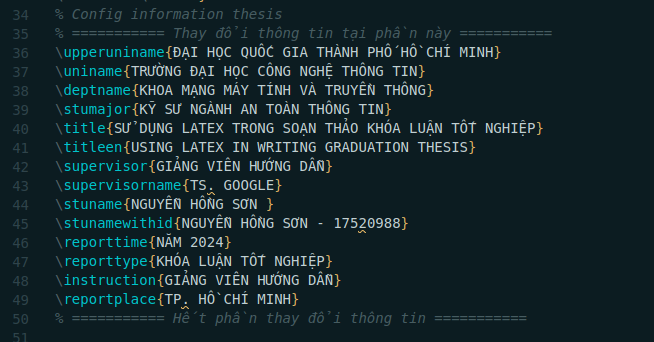
\includegraphics[scale=0.7]{chapter1/chap1-information-variable.png}
%     \caption{Phần thay đổi thông tin trang bìa}
%     \label{fig:chap1-information-variable}
% \end{figure}

% Các phần tiếp theo, quy định các nội dung được thêm vào báo cáo chính. Nếu một tập tin xuất hiện trong thư mục chapters nhưng không được khai báo bằng lệnh \textit{include} thì cũng không xuất hiện trong báo cáo. Vậy nên các chương mới bắt buộc phải được khai báo trong \textit{thesis.tex}. Các phần tài liêu tham khảo cũng được hiểu tương tự.

\chapter{Tổng quan}
\label{chap:chap1}
\section{Giới thiệu}
Công nghệ số chính là động lực cốt lõi, tạo ra một cú hích cho sự ra đời và phát triển thần tốc của các khóa học trực tuyến mở (MOOCs). Các nền tảng này đang từng bước định hình lại toàn cảnh giáo dục hiện đại thông qua tính linh hoạt, sự tiện lợi và khả năng tiếp cận không giới hạn. Làn sóng giáo dục trực tuyến này đang tạo ra một cuộc dịch chuyển trong tiêu chuẩn giáo dục toàn cầu, khẳng định vị thế của nó như một phương thức học tập ngày càng chủ đạo.

Tuy nhiên, tỷ lệ người học bỏ cuộc ở các khóa học MOOCs vẫn ở mức rất cao. Hiện tượng này không chỉ chứng tỏ các giới hạn của hệ thống mà sâu xa hơn, nó cho thấy sự thiếu kết nối hiệu quả giữa nội dung khóa học và người học. Sở dĩ có thực trạng này là do sự tác động từ hai nhóm nguyên nhân chính. Về phía nền tảng, cấu trúc học liệu đôi khi còn cồng kềnh, gây quá tải và môi trường học tập thiếu tính tương tác, hấp dẫn. Về phía người học, rào cản đến từ sự thiếu hụt kỹ năng học tập tự chủ, động lực không bền vững và thiếu một định hướng học tập rõ ràng. Trước thực trạng trên, việc đề ra các giải pháp nhằm hạ thấp tỷ lệ bỏ học là vô cùng cấp thiết.

Trong bối cảnh đó, việc phát triển các mô hình có khả năng dự đoán chính xác nguy cơ bỏ học của sinh viên được xem là một chiến lược can thiệp sớm đầy tiềm năng. Bằng việc nhận diện sớm các dấu hiệu hành vi bất thường, hệ thống có thể hỗ trợ cá nhân hóa lộ trình học, điều chỉnh phương pháp dạy, hoặc tăng cường mức độ tương tác. Mặc dù vậy, tồn tại không ít rào cản đáng kể về mặt kỹ thuật, cụ thể là:
\begin{enumerate}
    \item \textbf{Khối lượng dữ liệu khổng lồ và đa dạng của MOOCCubeX:} Dữ liệu được lấy từ các nền tảng MOOCs rất lớn, trong đó thông tin về khóa học, hồ sơ người dùng, lịch sử học tập, tương tác với nội dung và với những người học khác. Bên cạnh đó, dữ liệu có tính chất đa dạng: từ dữ liệu có cấu trúc, bán cấu trúc và không cấu trúc. Trước những đặc tính này, yêu cầu cốt lõi đặt ra là khả năng xử lý đồng thời nhiều định dạng dữ liệu khác nhau với tốc độ cao và độ chính xác tuyệt đối cùng với khối lượng dữ liệu lớn. Hệ thống cần sở hữu nền tảng mở rộng linh hoạt (scalable) để thích ứng với tốc độ sinh dữ liệu, cùng cơ chế tích hợp liền mạch cho phép đồng bộ đa nguồn thời gian thực. 

    \item \textbf{Tính không hoàn chỉnh và thiếu đồng nhất của dữ liệu:} Trong môi trường MOOC, việc người học bỏ dở khóa học giữa chừng, không hoàn thành bài kiểm tra, hoặc bỏ qua các nội dung học tập dẫn đến tình trạng dữ liệu bị phân mảnh và thiếu hụt nghiêm trọng. Thêm vào đó, nguyên nhân từ những bất cập trong quy trình thu thập và lưu trữ cũng là lý do. Sự thiếu hụt dữ liệu ảnh hưởng trực tiếp đến tính toàn vẹn và đồng nhất của bộ dữ liệu.
\end{enumerate}

Xuất phát từ những thách thức trên, nghiên cứu này đề xuất và phát triển các mô hình học sâu cho bài toán dự đoán kết quả hoàn thành khóa học của người học trên MOOCs. Cụ thể, nghiên cứu nhằm đạt được hai mục tiêu sau:
\begin{enumerate}
    \item Giải quyết thách thức dữ liệu lớn và không đầy đủ trên MOOCs: Mục tiêu này tập trung vào việc xử lý dữ liệu lớn, không đầy đủ thông qua việc tích hợp các kỹ thuật xử lý tiền kỳ như làm sạch, chuẩn hóa và đặc biệt là điền khuyết dữ liệu. Khóa luận đề xuất một giải pháp tiên tiến để suy diễn dữ liệu thiếu bằng GCN, cho phép khai thác hiệu quả cấu trúc quan hệ tiềm ẩn giữa các thực thể học tập (ví dụ: sinh viên, bài giảng, tương tác).
    
    \item Dự đoán kết quả hoàn thành khóa học trên MOOCs: Ứng dụng các mô hình học sâu nhằm khai thác hiệu quả dữ liệu học tập phong phú trong MOOCs, từ hành vi truy cập, lịch sử học tập đến mức độ tương tác với nội dung. Khóa luận này sử dụng 4 mô hình học sâu bao gồm: RNN, GRU, 4-layer stacked LSTM, BiLSTM.
\end{enumerate}
Chúng tôi mong muốn với những mục tiêu trên, khóa luận sẽ đem lại ý nghĩa trong việc nâng cao tỷ lệ duy trì học tập, giảm thiểu tình trạng bỏ học. Qua đó, giúp người học khai thác tối đa tiềm năng của các nền tảng MOOCs và mở rộng cơ hội tiếp cận tri thức.


% Trong bối cảnh hiện đại, giáo dục đã có cách mạng lớn đó là hệ thống giáo dục trực tuyến hiện đại. Hệ thống giáo dục hiện đại chứng kiến sự ra đời và phát triển mạnh mẽ của các nền tảng học trực tuyến mở (MOOC), mở ra vô vàn cơ hội tiếp cận tri thức cho mọi đối tượng đến từ mọi nơi trên thế giới thông qua giảng dạy trực tuyến. Để thực hiện trên quy mô lớn này, các hệ thống giáo dục này luôn có kho tàng khổng lồ các khoá học phong phú, đa dạng để đáp ứng cho nhiều đối tượng người học. Do đó, người học thường xuyên gặp khó khăn trong việc xác định, chọn lựa môn học phù hợp với mong muốn và năng lực của bản thân. Để giải quyết thực trạng này, việc nghiên cứu và xây dựng một hệ thống khuyến nghị môn học hiệu quả cho các nền tảng MOOC là hết sức cần thiết để giải quyết các thực trạng sau:

% Trong bối cảnh giáo dục hiện đại, hệ thống khuyến nghị đã chứng minh được giá trị của mình bằng cách cung cấp các gợi ý phù hợp cho các cơ sở giáo dục, giáo viên và học sinh. Đặc biệt, với sự bùng nổ của các nền tảng MOOC, việc xây dựng một hệ thống khuyến nghị môn học hiệu quả trở thành một nhu cầu cấp thiết.

% Nhằm giải quyết các thách thức lớn nêu trên và khai thác hiệu quả dữ liệu Big Data từ các nền tảng MOOC, tác giả đề xuất đề tài "Nghiên cứu phương pháp cải tiến hệ thống khuyến nghị môn học dựa trên dữ liệu lớn từ các nền tảng MOOC" với hai mục tiêu chính:
% \begin{enumerate}
%     \item Tập trung giải quyết các thách thức từ dữ liệu lớn từ MOOC. Xử lý và khai thác dữ liệu hiệu quả, mô hình hoá các tương tác của người dùng để thu được dữ liệu có ích để nắm bắt được sở thích, tính cá nhân hoá của người dùng.
%     \item Xây dựng hệ thống khuyến nghị hiện đại, tận dụng dữ liệu lớn từ MOOC để đề xuất môn học phù hợp với từng người dùng.
% \end{enumerate}

\section{Bài toán nghiên cứu}
Với những ưu điểm về tính linh hoạt, tiện lợi và khả năng tiếp cận trên quy mô lớn, các nền tảng MOOCs đã khẳng định vị thế mạnh mẽ. Vượt ra ngoài chức năng là một không gian học tập độc lập, MOOCs hiện nay còn được tích hợp sâu rộng vào giáo dục bậc đại học, hình thành nên các mô hình học tập kết hợp (Blended Learning - BL) năng động, đáp ứng hiệu quả nhu cầu đa dạng của người học trong thời đại số \cite{de2021use}.

Hew và cộng sự (2014) \cite{hew2014students} đã chỉ ra ba nhóm động lực chính của người học. Thứ nhất là nhu cầu trau dồi tri thức, bao gồm việc khám phá các lĩnh vực mới hoặc đào sâu chuyên môn. Thứ hai là mong muốn chinh phục các thử thách cá nhân và kiểm chứng năng lực bản thân. Thứ ba là mục tiêu thu thập các chứng chỉ nhằm phục vụ cho việc học tập lên cao hoặc phát triển sự nghiệp. Sự đa dạng trong các động cơ này cho thấy tiềm năng to lớn của MOOCs trong việc đáp ứng một phổ rộng các mục tiêu giáo dục cá nhân.

Một đặc điểm ưu việt khác của MOOCs so với giáo dục truyền thống là khả năng thu thập và phân tích dữ liệu học tập ở quy mô lớn. Ví dụ thời lượng tương tác với video bài giảng, tiến độ hoàn thành bài tập, mức độ tham gia diễn đàn và kết quả cuối kỳ đều được ghi nhận. Nguồn dữ liệu lớn (big data) này mở ra cơ hội để nhận diện các xu hướng học tập, giúp phát hiện sớm các dấu hiệu có nguy cơ bỏ học, từ đó có các biện pháp can thiệp kịp thời.

Một trong những rào cản lớn khiến người học chùn bước là khó khăn khi tương tác trong một ngôn ngữ khác biệt, đặc biệt đối với những người học đến từ các nước không sử dụng tiếng Anh. Khi tương tác với người học khác trong môi trường trực tuyến toàn cầu, những rào cản này có thể làm tăng sự khó khăn trong giao tiếp, trao đổi ý tưởng và tiếp thu kiến thức \cite{ma2023leveraging}.

Thực tế cho thấy, chỉ khoảng 10\% số người đăng ký hoặc thậm chí ít hơn hoàn thành các khóa học phổ biến \cite{hew2014students}. Nhiều nguyên nhân đã được chỉ ra, bao gồm: thiếu động lực học tập bền vững, thiếu kiến thức nền tảng cần thiết để theo kịp nội dung, sự không tập trung vào diễn đàn tương tác, khó hiểu bài giảng khi thiếu hỗ trợ kịp thời, yêu cầu khóa học mơ hồ, và đặc biệt là không đủ thời gian do các ưu tiên khác trong cuộc sống, dẫn đến tình trạng trì hoãn và cuối cùng là bỏ cuộc.

Chính vì đó, trong thời gian qua, các nhà nghiên cứu xem xét một cách toàn diện nhiều yếu tố, từ đặc điểm cụ thể của từng khóa học, trường đại học, nền tảng công nghệ cung cấp MOOC, cho đến hồ sơ và đặc điểm cá nhân của người học. Mục tiêu cuối cùng là tìm ra những yếu tố chính dẫn đến quyết định hoàn thành hay bỏ dở khóa học của người học. Việc xác định sớm kết quả hoàn thành khóa học và có cơ chế can thiệp kịp thời để giảm thiểu nguy cơ tiềm ẩn đã được chứng minh là những giải pháp then chốt giúp giải quyết thách thức này.\cite{baneres2023early, andres2018studying}.
\begin{figure}[H]
    \centering
    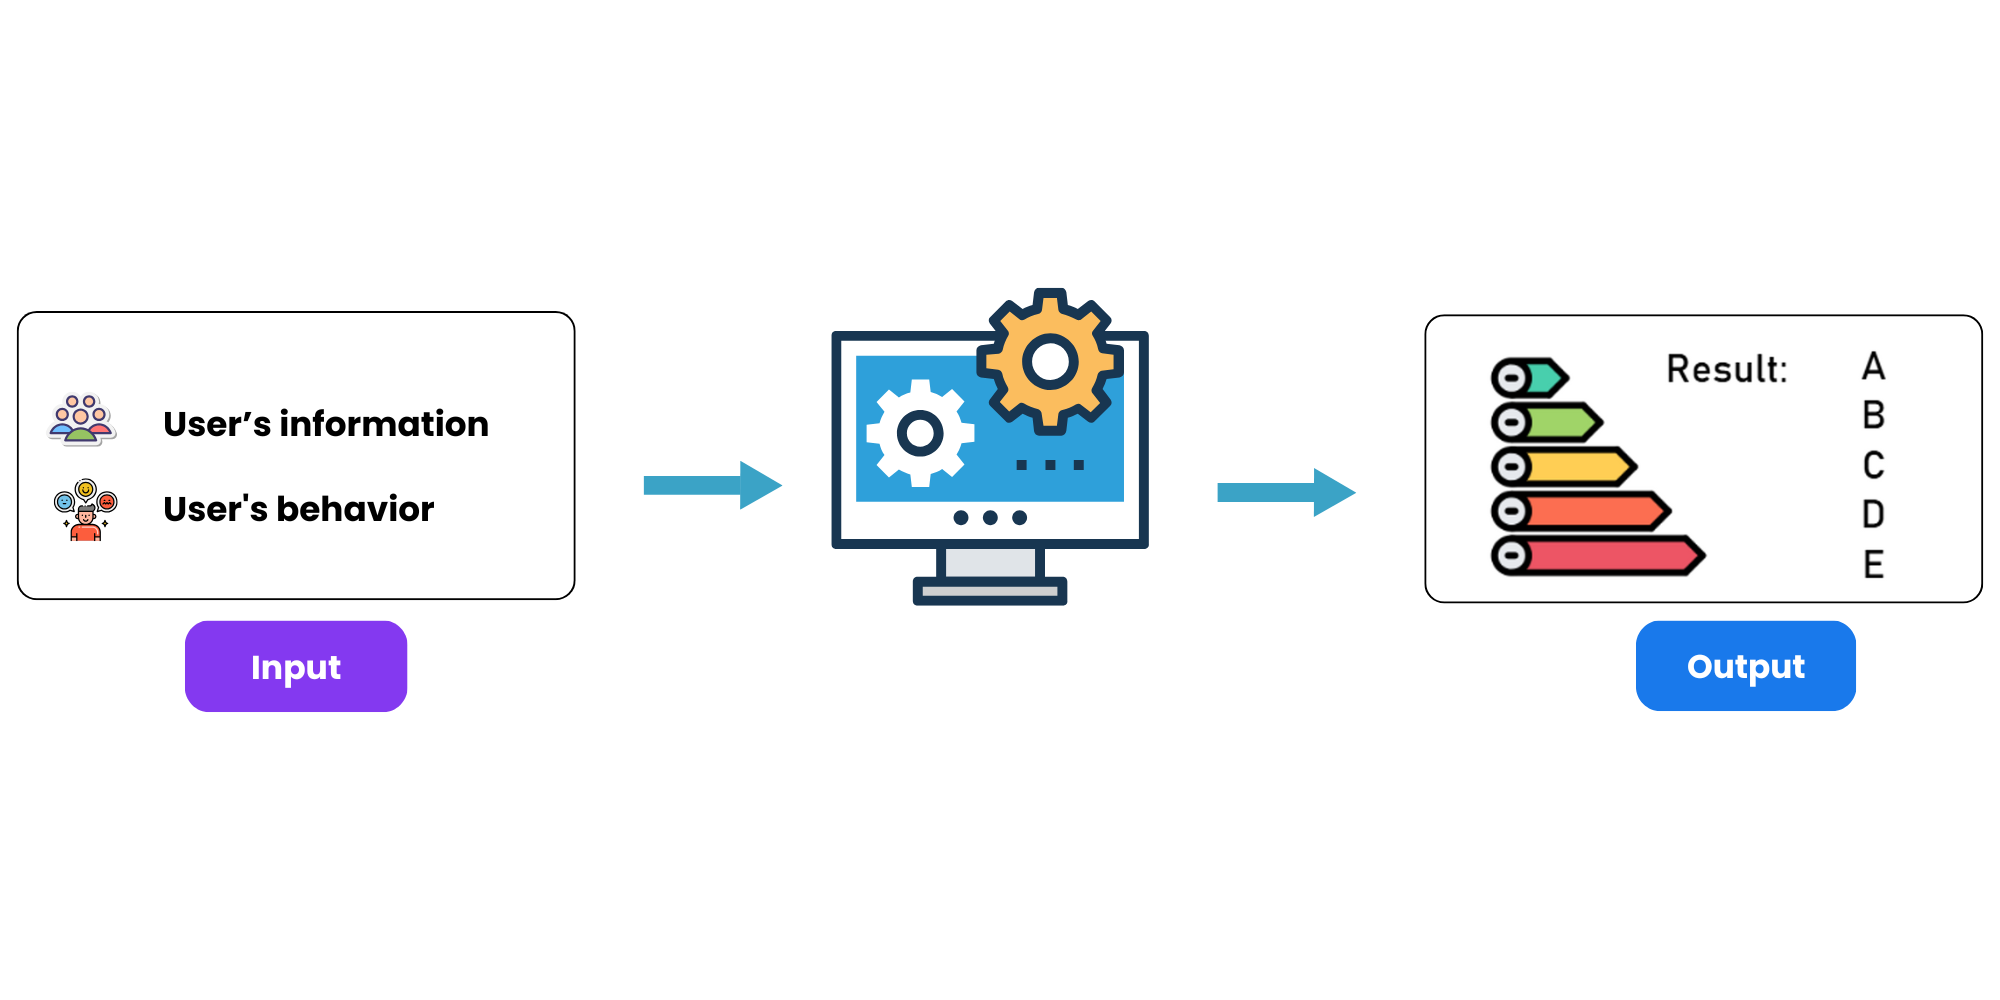
\includegraphics[width = 0.8\textwidth]{imgs/input-output.png}
    \caption{Minh hoạ input và output của bài toán.}
    \label{fig:input_output}
\end{figure}

Bài toán mà chúng tôi đặt ra là dự đoán kết quả hoàn thành khóa học và đưa ra cảnh báo sớm trên các nền tảng MOOCs dựa trên dữ liệu học tập của học viên. Cụ thể như sau:

\begin{itemize}
    \item \textbf{Input:} Dữ liệu học tập của học viên, bao gồm hành vi học tập (thời gian học, số bài tập đã hoàn thành, điểm số), đặc điểm cá nhân, thông tin khóa học, thời gian hoàn thành bài tập và hành vi tương tác (số lần bình luận, phản hồi trên diễn đàn).

    \item \textbf{Output:} Dự đoán kết quả hoàn thành khóa học của người học phân loại theo 5 cấp độ (A: Xuất sắc, B: Giỏi, C: Đạt yêu cầu, D: Không đạt, E: Chưa hoàn thành).
\end{itemize}
Nguồn dữ liệu từ nền tảng MOOC thường có tỷ lệ dữ liệu bị khuyết rất cao, thậm chí lên đến hơn 60\%. Tình trạng này gây trở ngại trong việc xử lý và nắm bắt hành vi người học, song song đó còn làm giảm đáng kể hiệu suất mô hình học sâu, vốn rất nhạy cảm với sự thiếu hụt dữ liệu.

Để giải quyết thách thức về dữ liệu thiếu, khóa luận này triển khai Mạng đồ thị tích chập (GCN) như một phương pháp cốt lõi để suy diễn và bổ sung các giá trị khuyết. Cách tiếp cận này vượt trội hơn so với các kỹ thuật truyền thống vốn xử lý từng điểm dữ liệu một cách độc lập. Thay vào đó, GCN cho phép khai thác cấu trúc quan hệ phức tạp giữa các thực thể như sinh viên, hoạt động học tập và đặc điểm khóa học, từ đó đưa ra các dự đoán về giá trị thiếu một cách thông minh và chuẩn xác hơn. Việc áp dụng GCN mang lại lợi ích kép: vừa nâng cao chất lượng dữ liệu đầu vào, vừa tạo tiền đề thuận lợi để cải thiện hiệu suất dự báo của các mô hình học sâu. Khi dữ liệu được xử lý một cách toàn diện, các pipeline học sâu có thể "học" được hành vi người dùng hiệu quả hơn, dẫn đến khả năng dự báo chính xác về kết quả học tập, mức độ gắn kết và nguy cơ bỏ học.

% Cấu trúc của các phần còn lại trong khóa luận được tổ chức như sau. Đầu tiên, chúng tôi sẽ đi sâu vào việc phân tích nền tảng lý thuyết và các công trình liên quan đến bài toán dự đoán kết quả học tập. Tiếp theo, một chương riêng sẽ trình bày chi tiết quá trình thực nghiệm và kết quả đánh giá, nhằm chứng minh hiệu quả vượt trội của phương pháp GCN trong bối cảnh dữ liệu MOOCs. Cuối cùng, phần kết luận sẽ tóm lược những đóng góp chính của nghiên cứu và đề xuất các hướng phát triển trong tương lai.

\section{Mục tiêu}

 Phương pháp GCN-I được kỳ vọng sẽ cải thiện chất lượng dữ liệu đầu vào, từ đó cải thiện đáng kể độ chính xác của mô hình. Bằng cách xử lý hiệu quả các giá trị thiếu hụt, mô hình có thể tận dụng tối đa thông tin sẵn có, giúp dự đoán trở nên tin cậy và chính xác hơn.

Các mục tiêu cụ thể của khóa luận được triển khai qua bốn giai đoạn chính như sau:
\begin{enumerate}
    \item \textbf{Khảo sát các phương pháp hiện tại}: Giai đoạn đầu sẽ thực hiện một tổng quan lý thuyết sâu rộng về các công trình hiện có. Trọng tâm là phân tích các pipeline học sâu và các phương pháp điền khuyết dữ liệu đã được áp dụng trên nền tảng MOOCs. Quá trình này giúp hiểu rõ đặc điểm cấu trúc, nguyên lý hoạt động, điểm mạnh và thiếu sót của mô hình. Việc phân tích sâu sắc các phương pháp hiện tại không chỉ làm rõ các phương pháp hiện có và là nền tảng cho nghiên cứu, mà còn giúp xác định khoảng trống nghiên cứu và tiếp cận bài toán theo cách đúng đắn và phù hợp.
    \item \textbf{Khai phá và phân tích đặc trưng dữ liệu MOOCs}: Giai đoạn này khai thác và phân tích chuyên sâu bộ dữ liệu quy mô lớn từ nền tảng MOOCs. Quy trình bao gồm các bước thu thập, tiền xử lý và phân tích, nhằm trích xuất những thông tin cốt lõi liên quan đến hành vi người học. Mục tiêu là nhận diện các đặc trưng nổi bật và các xu hướng học tập tiềm ẩn, từ đó đề xuất các phương pháp xử lý và phân tích dữ liệu hiệu quả, có định hướng rõ ràng.

    \item \textbf{Đề xuất và triển khai phương pháp cải thiện dữ liệu}: Dựa trên các đặc điểm dữ liệu và tổng hợp từ các công trình đi trước, khóa luận đề xuất GCN-I, một phương pháp điền khuyết dữ liệu dựa trên đồ thị. Phương pháp này tận dụng khả năng lan truyền thông tin giữa các nút lân cận trong cấu trúc đồ thị để suy luận và điền vào các giá trị bị thiếu một cách chuẩn xác.

    \item \textbf{Thiết kế kịch bản thực nghiệm và đánh giá hiệu năng}: Giai đoạn cuối cùng của khóa luận tập trung vào việc xây dựng và thực thi các kịch bản thực nghiệm để kiểm chứng và định lượng hiệu quả của phương pháp đã đề xuất. Quá trình đánh giá sẽ được tiến hành trên cả hai khía cạnh: chất lượng dữ liệu sau khi xử lý và hiệu suất của mô hình dự đoán. Các kết quả thu được không chỉ nhằm định lượng mức độ cải thiện về độ chính xác và khả năng khái quát hóa, mà còn góp phần khẳng định giá trị và tiềm năng ứng dụng thực tiễn của GCN-I trong bối cảnh dữ liệu lớn và thưa thớt.
\end{enumerate}
\section{Phạm vi và đối tượng nghiên cứu}
% \subsection{Bộ dữ liệu MOOCCubeX}
Đề tài nghiên cứu tập trung vào việc cải thiện chất lượng dữ liệu nhằm nâng cao kết quả dự đoán của các mô hình học sâu trong bài toán dự đoán kết quả hoàn thành khóa học của người học trên nền tảng MOOCs. Nghiên cứu tích hợp hệ thống nhãn đánh giá toàn diện và ứng dụng các thư viện, công cụ hàng đầu như scikit-learn, TensorFlow, Keras và PyTorch. Chúng tôi sử dụng bộ dữ liệu được cung cấp từ XueTangX - nền tảng học tập trực tuyến của Trung Quốc trong giai đoạn 2019-2020.

Đối tượng nghiên cứu là người học tham gia học tập trên nền tảng MOOCs, dữ liệu thu thập bao gồm thông tin nhân khẩu học vả hành vi học tập. Tập dữ liệu tổng hợp quy mô lớn với 4.216 khóa học, 230.263 video giảng dạy, 358.265 bài tập, 637.572 khái niệm học tập chi tiết cùng hơn 296 triệu bản ghi hành vi thô từ 3.330.294 người học.

\section{Cấu trúc báo cáo khóa luận}
Cấu trúc của khóa luận bao gồm 7 chương chính, được trình bày như sau:

\begin{itemize}
\item \textbf{Chương \ref{chap:chap1} - Tổng quan:} Trình bày bối cảnh, mục tiêu, phạm vi, đối tượng nghiên cứu và cấu trúc khóa luận.
\item \textbf{Chương \ref{chap:chap2} - Các công trình nghiên cứu liên quan:} Tổng hợp các công trình tiêu biểu về mạng nơ-ron đồ thị và học sâu.
 \item \textbf{Chương \ref{chap:chap3} - Cơ sở lý thuyết:} Cung cấp kiến thức nền về học sâu, GCN và các phương pháp làm giàu dữ liệu.
\item \textbf{Chương \ref{chap:chap4} - GCN-I: Phương pháp suy diễn giá trị khuyết:} Giới thiệu, bộ dữ liệu thực nghiệm và trình bày phương pháp đề xuất.
\item \textbf{Chương \ref{chap:chap5} - Thực nghiệm và đánh giá:} Mô tả quá trình thực nghiệm, chỉ số đánh giá và kết quả thực nghiệm.
\item \textbf{Chương \ref{chap:chap6} - SmartEduTrack:} Giới thiệu hệ thống hỗ trợ theo dõi học tập thông minh nhằm phục vụ quản lý giáo dục.
\item \textbf{Chương \ref{chap:chap7} - Kết luận và hướng phát triển:} Tổng kết những đóng góp chính và đề xuất các hướng nghiên cứu trong tương lai.
 \item \textbf{Tài liệu tham khảo:} Danh mục các công trình đã được trích dẫn trong khóa luận.
\end{itemize}
 
 % Nghiên cứu này sẽ sử dụng dữ liệu từ các nền tảng MOOCs thực tế như Coursera\footnote{https://www.coursera.org/}, edX\footnote{https://www.edx.org/}, XuetangX\footnote{https://www.xuetangx.com/},... để đảm bảo tính thực tiễn khi đánh giá.
% \subsection{Các kiến trúc dữ liệu lớn}
% Khoá luận tập khảo sát và ứng dụng các kiến trúc dữ liệu lớn hiện đại. Các kiến trúc này được xây dựng trên nền tảng của nhiều công nghệ và thành phần khác nhau, kết hợp chặt chẽ để giải quyết các thách thức đặc thù của dữ liệu lớn. Việc thiết kế kiến trúc dữ liệu lớn đòi hỏi sự cân nhắc kỹ lưỡng về hiệu năng, khả năng mở rộng, tính linh hoạt và bảo mật. Các thành phần phổ biến của một kiến trúc dữ liệu lớn bao gồm nguồn dữ liệu, hệ thống lưu trữ, xử lý dữ liệu theo lô và theo luồng, kho dữ liệu phân tích, phân tích và báo cáo, và điều phối. 
 
%  Một số kiến trúc dữ liệu lớn phổ biến hiện nay có thể kể đến như Data Warehouse, Data Lake và Data Lakehouse.
    
% \subsection{Mô hình khuyến nghị}
% nghiên cứu sẽ tập trung vào phát triển và cải tiến các mô hình khuyến nghị môn học. Đây là những thuật toán học máy hoặc học sâu phức tạp, có khả năng dự đoán sở thích và mức độ phù hợp của người dùng với các khóa học khác nhau, dựa trên dữ liệu về người dùng, khóa học và tương tác của họ. Các mô hình này thường được phân loại theo phương pháp tiếp cận, bao gồm lọc cộng tác, lọc dựa trên nội dung và các phương pháp kết hợp. 

% Nghiên cứu này tập trung vào các mô hình khuyến nghị tuần tự như SASRec\cite{sasrec} và BERT4Rec\cite{bert} đồng thời cũng đánh giá với các mô hình cổ điển như BPR\cite{bpr} và NCF\cite{ncf}.
